\section{Contexto de la asociación}
\label{sec:asociacion}

\subsection{Quiénes son}

\begin{wrapfigure}{r}{0.5\textwidth}
    \centering
    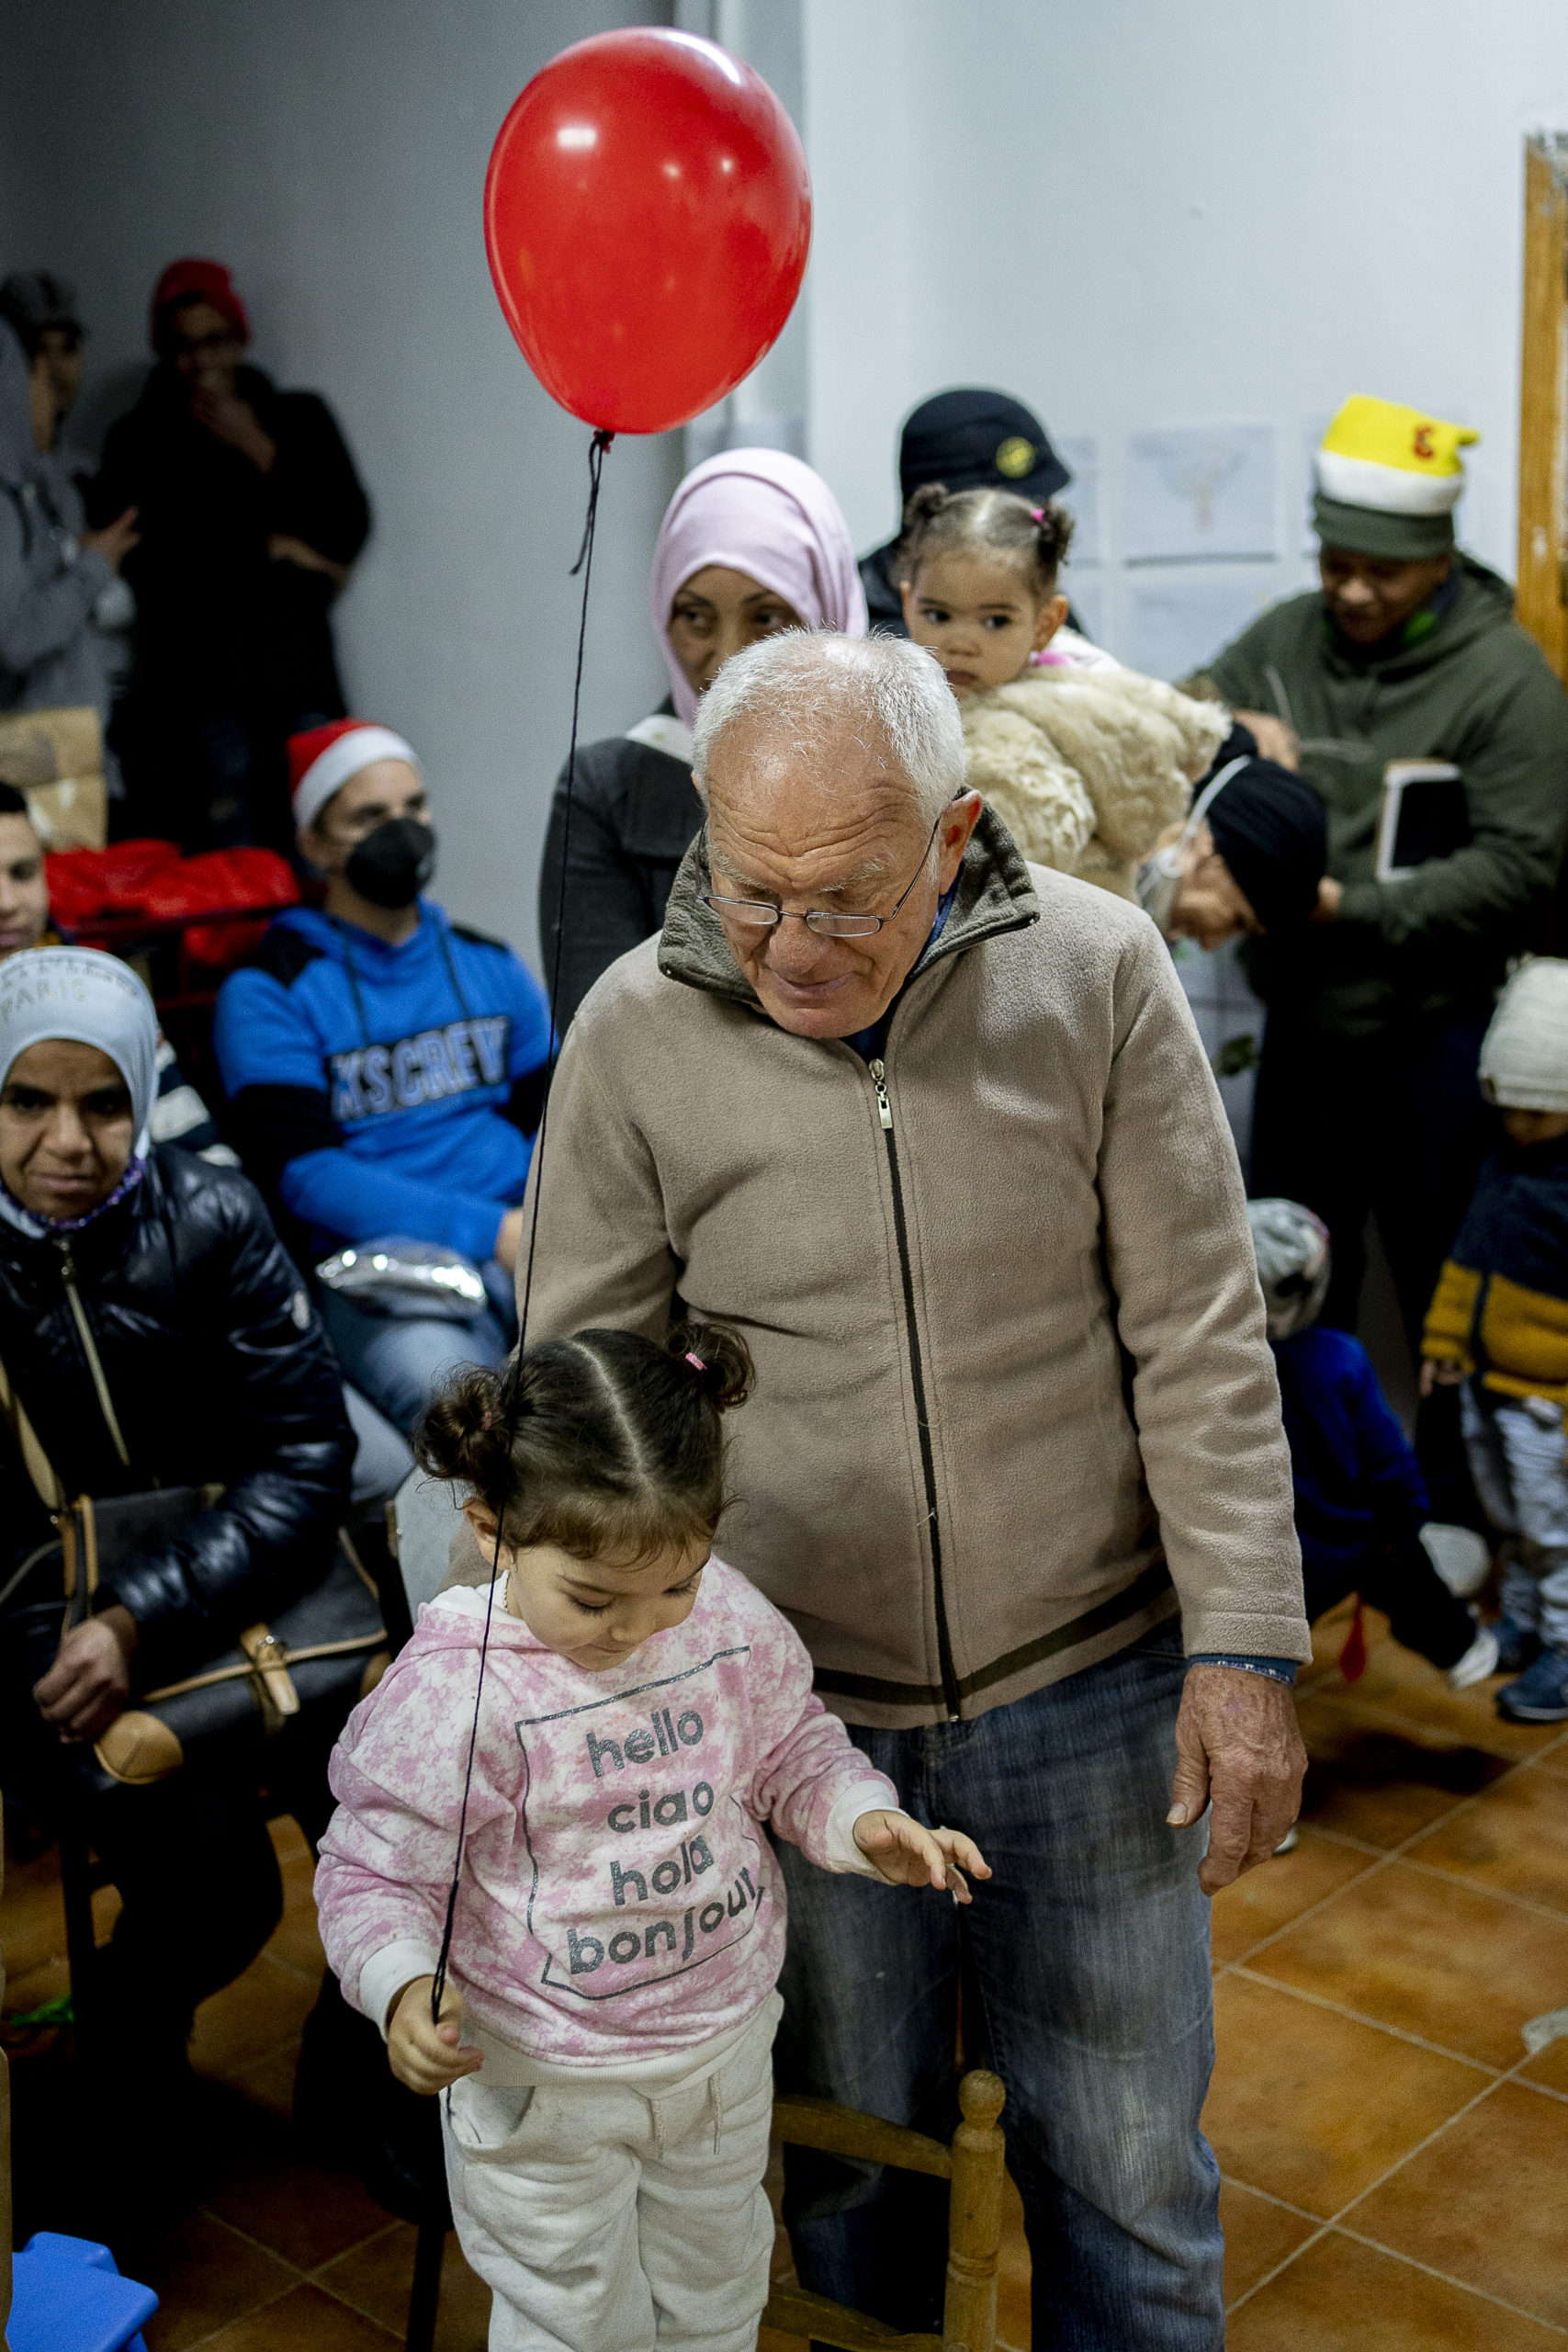
\includegraphics[width=0.9\linewidth]{imagenes/fes/gente.jpg}
\end{wrapfigure}

La \textit{Fundación Escuela de Solidaridad} busca ``recuperar el sentido familiar de personas que, por diversas circunstancias, no han podido ni pueden experimentarlo'' \cite{web-feds}. Esto lo consiguen principalmente mediante la acogida de cientos de personas de forma altruista. En su mayoría, están dirigidos a personas con riesgo de exclusión social, donde entran tanto familias al completo, como personas con casos más específicos.

Con esto, la asociación pretende que estas personas encuentren un lugar donde desarrollarse personalmente, pudiendo hacer frente mediante la ayuda colectiva, a mejorar y revertir sus situaciones personales. Todo esto lo hacen mediante el trabajo de cientos de voluntarios, así como personas que dedican el 100\% de su tiempo a la fundación.

La convivencia y el correcto funcionamiento de la fundación viene dado por la colaboración colectiva de todas las personas pertenecientes a esta. Tanto voluntarios como convivientes realizan tareas u obligaciones comunales dentro de sus capacidades y conocimientos, tanto para aportar valor a la convivencia, así como fomentar su inserción socio/laboral. Las estancias en la fundación no atienden al tiempo, si no al correcto desarrollo de las personas. Estas la abandonan en el momento en el que su situación lo permita. Actualmente, cuentan con más de 100 personas conviviendo, algunas de forma permanente y otras de corta estancia, generalmente voluntarios.

\subsection{Cómo trabajan}

\textit{Fundación Escuela de Solidaridad} está principalmente dirigida por dos organizadores permanentes, Dora e Ignacio. Aun siendo un equipo pequeño y con mucho trabajo que realizar consiguen llevar el proyecto adelante con la ayuda de voluntarios temporales. El número de voluntarios suele variar según la época del año.

Tanto el trabajo como la organización de la fundación son realizados mediante herramientas no especializadas para este tipo de colectivos. Suelen trabajar con programas de ofimática, como son hojas de cálculo, que les ofrecen las características necesarias para un control de la fundación, pero no para todas las necesidades de esta. El trabajo con la información y el acceso rápido a ella, son algunas de las lacras que persiguen a su forma de trabajar.

\subsection{Actividades de la fundación}

\begin{wrapfigure}{r}{0.4\textwidth}
    \centering
    
\includegraphics[width=0.9\linewidth]{imagenes/fes/taller2.jpg}
\end{wrapfigure}

La principal actividad de la fundación es la ya comentada acogida de personas. Todo esto lo complementan con diversos programas dirigidos tanto a personas de la fundación como a externas. Estos programas se hacen a nivel local e internacional. En primer lugar los programas locales van desde programas dedicados a mejorar el nivel laboral de las personas hasta fomentar el arte de estas. A nivel internacional, realizan proyectos ERASMUS+ dedicados generalmente a formar a la gente en el ámbito de la ayuda social. Todos estos programas se complementan con la realización de talleres de todo tipo, dedicados a la formación de las personas en diferentes materias.